%  Add 'draft' option to mark overfull boxes with black boxes
%  Add 'showkeys' option to make keywords appear
\documentclass[
aps,
reprint,
amsmath, amssymb,
%preprint,
superscriptaddress,
%groupedaddress
]{revtex4-2}
\usepackage[spanish]{babel}
\usepackage{float}
\usepackage{graphicx}
\usepackage{dcolumn}
\usepackage{bm}
\usepackage{physics}
\renewcommand{\andname}{y}
\renewcommand{\spanishtablename}{Tabla}
\newcommand{\up}[1]{^{#1}}
\begin{document}
\preprint{Universidad de Córdoba}
% Use the \preprint command to place your local institutional report number in the upper righthand corner of the title page in preprint mode.
%\preprint{}

%Title of paper
\title{Análisis de las Propiedades de la Luz \\al Desplazarse en Diferentes Medios}

\author{Luis Miguel Patiño Buendía}
\author{Jesús Manuel Gallego Mercado}

\affiliation{Universidad de Córdoba.\\ Montería-Córdoba, Colombia}

%\email[]{Your e-mail address}
%\homepage[]{Your web page}
%\thanks{}


\date{\today}

\begin{abstract}
En el presente informe se estudió el comportamiento de un haz de luz que incide sobre una superficie que separa dos medios con propiedades distintas (tales como densidad, índice de refracción, etc). Específicamente, se estudió la irradiancia, la velocidad, los cambios de fase y las amplitudes de los haces transmitido y reflejado, con respecto al haz incidente al atravesar la interfase. Esto con el objetivo de corroborar el principio de conservación de energía mediante los conceptos de reflectancia y transmitancia,  determinar los índices de refraccción de algunos medios y relacionar cualitativamente los cambios de fase y las amplitudes de los haces (mediante un osciloscopio) sin analizar las componentes del campo eléctrico incidente. Para llevarlo a cabo, se utilizó el simulador Phet: "Reflexión y Refracción de la Luz", en el cual se hizo incidir mediante un láser, un haz de luz roja sobre diferentes medios (aire, vidrio, y materiales desconocidos). Con ayuda de los instrumentos de medida virtual, se tomaron datos de intensidad relativa, ángulos, y velocidades de los haces de luz. Se concluyó que el principio de conservación de energía está presente en la configuración de un haz de luz incidente sobre una superficie que separa dos medios. La intensidad del haz incidente se distribuye en una fracción de luz reflejada y otra transmitida, de manera que la suma de estas intensidades sea igual a la inicial. Esto se cumple de manera independiente de las propiedades de los medios en el cual se propaga el haz.
%REVISAR OBJETIVO
\end{abstract}


%\keywords{}
\maketitle
% References should be done using the \cite, \ref, and \label commands
\section{Introducción}
La luz, caracterizada como una onda electromagnética sufre fenómenos de onda tales como la reflexión y refracción que se pueden observar de forma directa y experimentalmente mediante haces de luz que se desplazan en medios diferentes; el tratamiento de estos fenómenos se abstrae de la conocida Ley de Snell, sin embargo, nos limitamos a estudiar exclusivamente las direcciones resultantes de los haces en función de los índices de refracción de los medios, pero obviamos la información sobre las propiedades de la onda electromagnética (como la velocidad, la irradancia, la amplitud, el cambio de fase, etc)  al incidir sobre una interfase. En este informe estudiaremos estas propiedades e intentaremos corroborar las relaciones que existen entre ellas.

\section{Reflexión y Refracción}
La reflexión y la refracción de la luz son dos fenómenos físicos que puede experimentar un rayo de luz. En la reflexión, el rayo de luz rebota sobre una superficie, mientras en la refracción el rayo de luz que pasa de un medio a otro cambia su ángulo de propagación.

\subsection{Reflexión de la Luz}

En la reflexión de la luz se puede distinguir el rayo original o rayo incidente y el rayo que se devuelve o rayo reflejado. En el punto donde el rayo incidente y el reflejado se encuentran, se traza una línea imaginaria perpendicular a la superficie que se conoce como normal.\\
\\
Entre el rayo incidente y la normal se forma el ángulo de incidencia, y entre la normal y el rayo reflejado se forma el ángulo de reflexión. Estos ángulos son iguales \cite{optics}.\\
\\
\subsubsection{Reflexión Interna Total}

Este fenómeno sólo se produce para ángulos de incidencia superiores a un cierto valor límite o crítico $\theta_c$ donde el rayo de luz refractado no es capaz de atravesar la superficie entre ambos medios y por ende se refleja completamente. La reflexión interna total solamente ocurre en rayos que viajan de un medio de alto índice refractivo hacia medios de menor índice de refracción. El ángulo límite o crítico viene dado por: 

\begin{align*}
    \theta_{c} = \sin^{-1}\left(\frac{n_{2}}{n_{1}}\right)
\end{align*}


\subsection{Refracción de la Luz}

La refracción de la luz se produce en la superficie de separación de los medios de diferente densidad;lo que afecta la velocidad de propagación de la luz. El desvío de la dirección de propagación será mayor a mayor diferencia de la velocidad de propagación en los dos medios.\\
\\
En la refracción de la luz se distingue el rayo incidente y el rayo refractado. Entre el rayo incidente y la línea normal se forma el ángulo de incidencia $\theta_i$. Mientras que entre el rayo refractado y la normal se forma el ángulo de refracción $\theta_t$ \cite{optics}.\\


\subsubsection{Leyes de la Refracción de la Luz}

\begin{itemize}
    \item Los índices de refracción $n_1$ y $n_2$, el ángulo de incidencia $\theta_{i}$ y el ángulo del haz refractado o transmitido $\theta_{t}$ se relacionan por la siguiente expresión:
    
    \begin{equation}
        \label{eqn:ley_snell}
        n_{1} \sin{\theta_{i}} = n_{2} \sin{\theta_{t}} 
    \end{equation}
\end{itemize}

\subsubsection{Índice de refracción}

Se denomina índice de refracción al cociente de la velocidad de la luz en el vacío y la velocidad de la luz en el medio cuyo índice se calcula. Se simboliza con la letra $n$ y se trata de un valor adimensional.

\begin{align}
\label{eqn:indice_r}
    n = \dfrac{c}{v}
\end{align}

Donde
\begin{itemize}
    \item $c =$ Velocidad de la luz en le vacío
    \item $v =$ Velocidad de la luz en el medio cuyo índice se calcula (agua, vidrio, etc.)
\end{itemize}

\section{\label{sec:ref_tram}Reflectancia y Transmitancia}
La reflectancia es la fracción de radiación incidente reflejada por una superficie.
Se define la \textbf{reflectancia} $R$ como el cociente entre la potencia (o flujo) del haz reflejado y la potencia del haz incidente. Es decir:

\begin{gather*}
    R \equiv \frac{I_r A\cos{\theta_r}}{I_i A \cos{\theta_i}} = \frac{I_r}{I_i}
\end{gather*}
Solamente es considerada el área de la sección transversal de los haces incidente y reflejedo (como se observa en la figura \ref{fig:img1}).\\

\begin{figure}
    \centering
    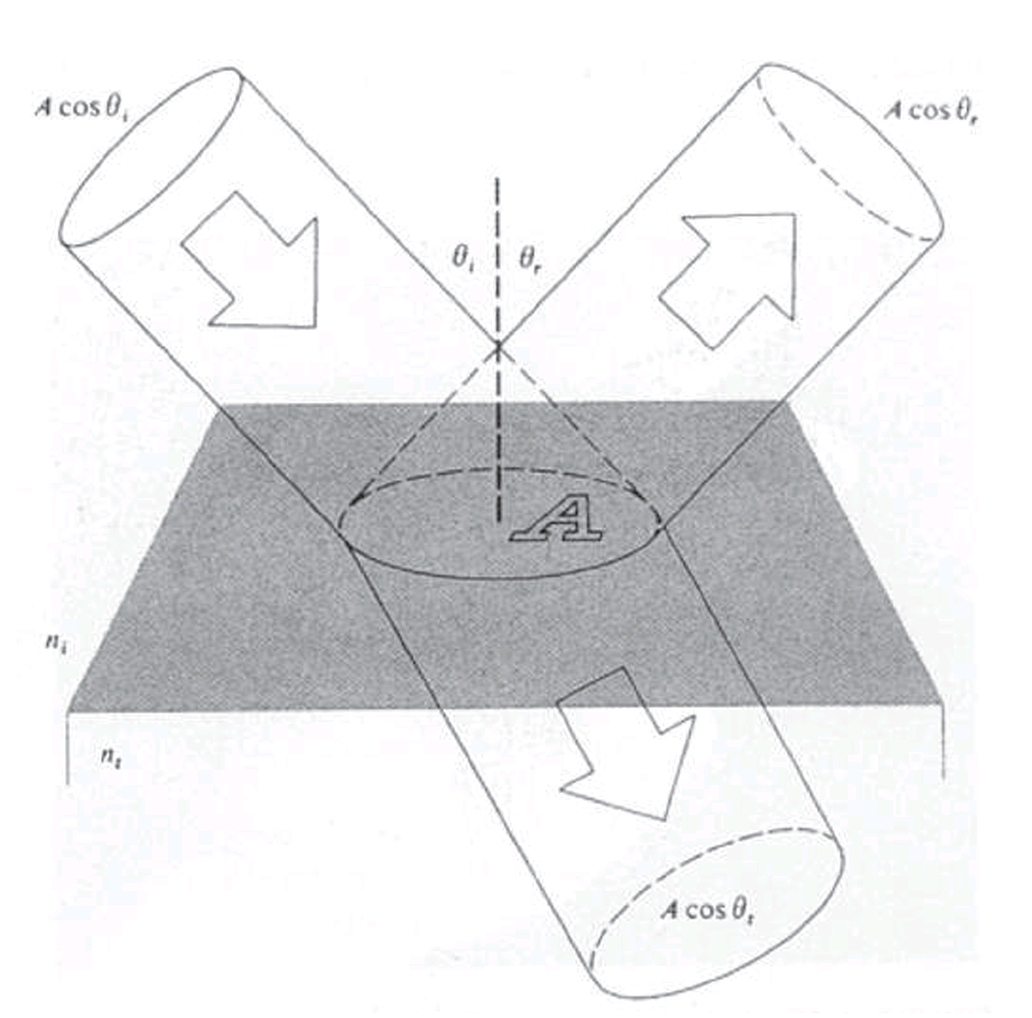
\includegraphics[width=0.8\columnwidth]{img/img1.jpg}
    \caption{Reflexión y transmisión de un haz incidente}
    \label{fig:img1}
\end{figure}

Mientras que la \textbf{transmitancia} $T$ se define como la fracción de luz incidente que pasa a través de una muestra, o también, el cociente entre el flujo transmitido y el flujo incidente:

\begin{gather*}
    T \equiv \frac{I_t \cos{\theta_t}}{I_i  \cos{\theta_i}} 
\end{gather*}

Los coeficientes de transmitancia y reflectancia satisfacen la relación:

\begin{gather}
\label{EQN:UNIDAD}
    R + T = 1
\end{gather}
\section{Objetivos}
\begin{enumerate}
    \item Estudiar las propiedades de la luz (tales como: velocidad, intensidad, amplitud y cambio de fase) al desplazarse en diferentes medios.
    \begin{itemize}
        \item Determinar la relación entre las intensidades de los haces reflejado y transmitido con respecto al haz incidente.
        \item Determinar la relación que existe entre la transmitancia y los índices de refracción de los medios.
        \item Analizar cualitativamente lo que ocurre con la fase y la amplitud del haz que se desplaza en dos medios distintos.
        \item Determinar los índices de refracción de algunos medios desconocidos del simulador Phet.
    \end{itemize}
\end{enumerate}

\section{\label{sec:expe}Experimento y Metodología}

El experimento se realizó mediante el simulador Phet: \textit{Bending Light} \footnote{Simulador Phet: Bending Light; Encontrado en internet: https://phet.colorado.edu/en/simulations/bending-light}. El montaje se puede observar mediante la figura \ref{fig:montaje}. Mientras que los materiales e instrumentos usados se encuentran en la tabla \ref{tab:materiales}.
\begin{table}[H]
	\caption{\label{tab:materiales}Materiales e Instrumentos de medida.}
	\begin{ruledtabular}
		\begin{tabular}{lcc}
            \textrm{Materiales} & \textrm{Referencia} & \textrm{Cantidad}\\
			\colrule
            Láser (rojo)                & --------- & 1\\
			Transportador    & --------- & 1\\
            Medidor virtual de Intensidad              & --------- & 1\\
            Medidor virtual de Rapidez   & --------- & 1\\
            Osciloscopio virtual & --------- & 1
	\end{tabular}
	\end{ruledtabular}
\end{table}

El experimento consistió en hacer incidir un haz de luz mediante un láser de luz roja sobre una interfase que inicialmente separa los medios aire $\rightarrow$ vidrio, se tomaron medidas de intensidad de luz, rapidez y distancia angular (con respecto a la recta normal) de los haces incidente, reflejado y transmitido. Posteriormente se midió (cualitativamente) qué ocurría con la amplitud y la fase de los haces con respecto al haz incidente. 

Este procedimiento se repitió 3 veces para diferentes medios con índices de refracción desconocidos que provee el simulador (denominados como \textbf{Misterio A} y \textbf{Misterio B}).

\begin{figure}
\centering
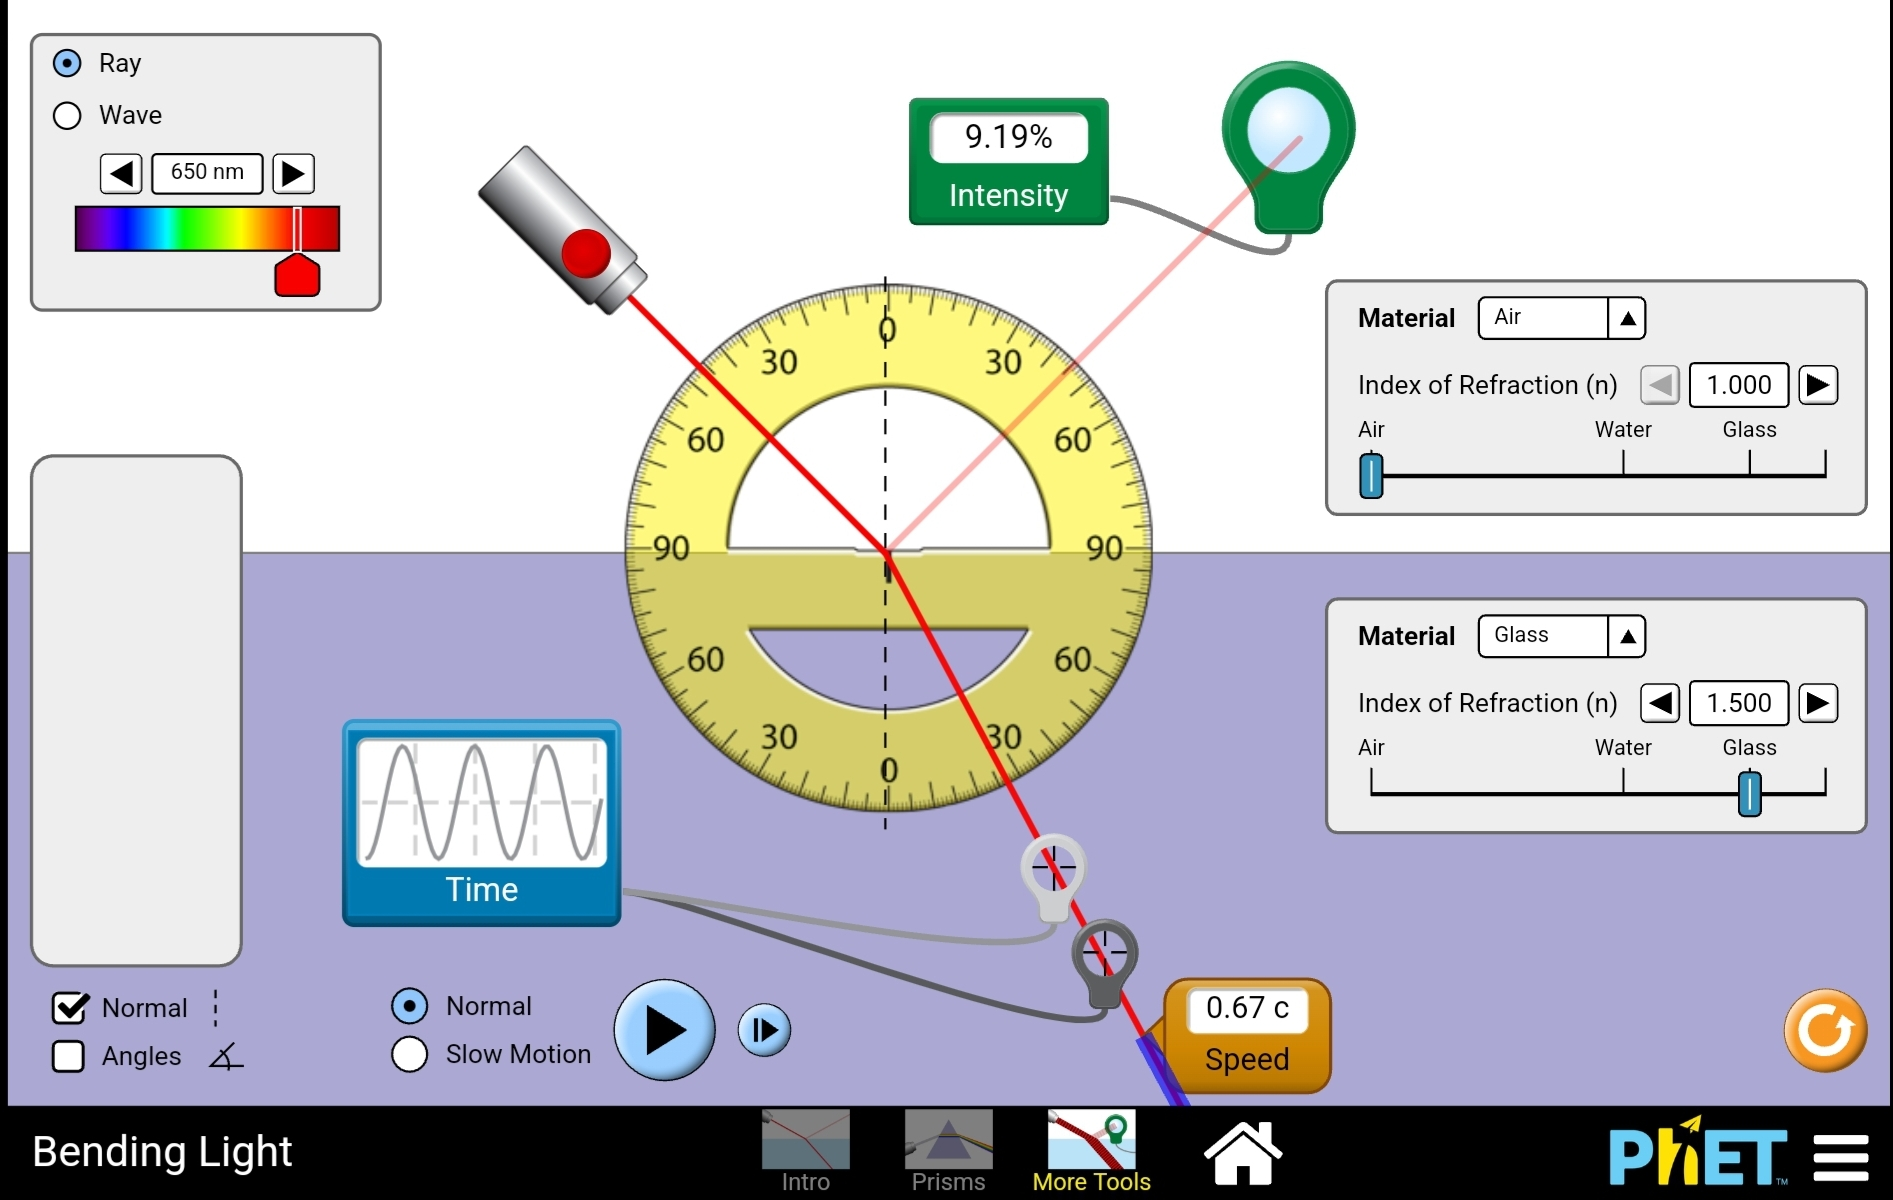
\includegraphics[width=\columnwidth]{img/montaje.jpg}
\caption{\label{fig:montaje} Montaje experimental: Reflexión y Refracción de la luz en el simulador Phet.}
\end{figure}

\section{\label{sec:resultados}Resultados}

Mediante cada tabla se consignan los datos medidos sobre el ángulo y la intensidad del haz incidente, reflejado y transmitido. Para efectos prácticos, la longitud de onda del simulador se fijó en $\lambda=650nm$, sin embargo, el color del haz de luz debía relacionarse con la frecuencia de la onda electromagnética, ya que al cambiar de medio de propagación, la rapidez de la onda cambia, simultáneamente la longitud de onda debería cambiar para mantener la frecuencia, y por ende el color del haz de luz intacto.
\begin{table}[H]%[H] add [H] placement to break table across pages
    \caption{\label{tab:tabla1}Haz que se desplaza en el medio: \textbf{aire al vidrio.} ($\lambda=650nm$ en el aire)}
     \begin{ruledtabular}
     \begin{tabular}{cc|cc|cc}
        \multicolumn{2}{c}{Haz Incidente}  & \multicolumn{2}{c}{Haz Reflejado} & \multicolumn{2}{c}{Haz Transmitido} \\
        \multicolumn{2}{c}{$v_i = 1c$}  & \multicolumn{2}{c}{$v_r=1c$} & \multicolumn{2}{c}{$v_t=0.67c$} \\
        \hline
        $\theta_i (^{\circ})$   & $I_{i}$(\%) & $\theta_r(^{\circ})$ & $I_{r}$(\%) & $\theta_t(^{\circ})$ & $I_{t}$(\%)\\
         0$^{\circ}$ & 100 & 0 $^{\circ}$ & 0.00  & 0 $^{\circ}$ & 96.01 \\
        14$^{\circ}$ & 100 & 14$^{\circ}$ & 4.32  & 9 $^{\circ}$ & 95.68 \\
        20$^{\circ}$ & 100 & 19$^{\circ}$ & 4.70  & 13 $^{\circ}$ & 95.30 \\
        30$^{\circ}$ & 100 & 30$^{\circ}$ & 5.63  & 18$^{\circ}$ & 94.37\\
        40$^{\circ}$ & 100 & 39$^{\circ}$ & 7.20  & 23$^{\circ}$ & 92.80\\
        60$^{\circ}$ & 100 & 60$^{\circ}$ & 16.20 & 33$^{\circ}$ & 83.80 \\
        80$^{\circ}$ & 100 & 79$^{\circ}$ & 46.29 & 39$^{\circ}$ & 53.71 \\
        \end{tabular}
     \end{ruledtabular}
\end{table}

\begin{table}[H]%[H] add [H] placement to break table across pages
    \caption{\label{tab:tabla2}Haz que se desplaza en el medio: \textbf{Misterio A, al aire.} ($\lambda=650nm$ en Misterio A)}
     \begin{ruledtabular}
     \begin{tabular}{cc|cc|cc}
        \multicolumn{2}{c}{Haz Incidente}  & \multicolumn{2}{c}{Haz Reflejado} & \multicolumn{2}{c}{Haz Transmitido} \\
        \multicolumn{2}{c}{$v_i = 0.41c$}  & \multicolumn{2}{c}{$v_r= 0.41c$} & \multicolumn{2}{c}{$v_t= 1c$} \\
        \hline
        $\theta_i (^{\circ})$   & $I_{i}$(\%) & $\theta_r(^{\circ})$ & $I_{r}$(\%) & $\theta_t(^{\circ})$ & $I_{t}$(\%)\\
         0$^{\circ}$ & 100 &  0$^{\circ}$ &  0.00 & 0 $^{\circ}$ &  82.78\\
         5$^{\circ}$ & 100 &  4$^{\circ}$ & 17.77 & 10 $^{\circ}$ & 82.23 \\
        11$^{\circ}$ & 100 &  9$^{\circ}$ & 19.86 & 23 $^{\circ}$ & 80.14 \\
        15$^{\circ}$ & 100 & 13$^{\circ}$ & 23.14 & 33$^{\circ}$ &  76.86\\
        20$^{\circ}$ & 100 & 20$^{\circ}$ & 34.65 & 52$^{\circ}$ &  65.35\\
        23$^{\circ}$ & 100 & 23$^{\circ}$ & 48.05 & 64$^{\circ}$ &  51.95 \\
        25$^{\circ}$ & 100 & 25$^{\circ}$ & 84.17 & 72$^{\circ}$ &  15.83 \\
        26$^{\circ}$ & 100 & 26$^{\circ}$ &100.00 & --$^{\circ}$ &  0
        \end{tabular}
     \end{ruledtabular}
\end{table}

\begin{table}[H]%[H] add [H] placement to break table across pages
    \caption{\label{tab:tabla3}Haz que se desplaza en el medio: \textbf{Misterio A al Misterio B} ($\lambda=650nm$ en el medio B)}
     \begin{ruledtabular}
     \begin{tabular}{cc|cc|cc}
        \multicolumn{2}{c}{Haz Incidente}  & \multicolumn{2}{c}{Haz Reflejado} & \multicolumn{2}{c}{Haz Transmitido} \\
        \multicolumn{2}{c}{$v_i = 0.71c$}  & \multicolumn{2}{c}{$v_r= 0.71c$} & \multicolumn{2}{c}{$v_t=0.41c$} \\
        \hline
        $\theta_i (^{\circ})$   & $I_{i}$(\%) & $\theta_r(^{\circ})$ & $I_{r}$(\%) & $\theta_t(^{\circ})$ & $I_{t}$(\%)\\
         0$^{\circ}$ & 100 &  0$^{\circ}$ &  0.00 & 0 $^{\circ}$ & 92.80 \\
        20$^{\circ}$ & 100 & 20$^{\circ}$ &  8.10 & 9 $^{\circ}$ & 91.90 \\
        30$^{\circ}$ & 100 & 31$^{\circ}$  & 9.60 & 16 $^{\circ}$ &90.40 \\
        40$^{\circ}$ & 100 & 40$^{\circ}$ & 12.00 & 20$^{\circ}$ & 88.00\\
        60$^{\circ}$ & 100 & 61$^{\circ}$ & 23.32 & 28$^{\circ}$ & 76.68\\
        85$^{\circ}$ & 100 & 85$^{\circ}$ & 69.51 & 33$^{\circ}$ & 30.49 \\
        \end{tabular}
     \end{ruledtabular}
\end{table}


\section{Análisis}

A partir de las tablas \ref{tab:tabla1}, \ref{tab:tabla2} y \ref{tab:tabla3} y la expresión (\ref{eqn:indice_r}), se calculan los índices de refracción de cada medio y se consignan en la tabla \ref{tab:indices}:

\begin{table}[H]%[H] add [H] placement to break table across pages
    \caption{\label{tab:indices}Índices de refracción calculados mediante la rapidez del haz en su medio correspondiente}
     \begin{ruledtabular}
     \begin{tabular}{lc}
      Medio Material & Índice de Refracción\\
      \hline
      Aire & 1.00\\
      Vidrio & 1.49\\
      Misterio A & 2.44\\
      Misterio B & 1.41
        \end{tabular}
     \end{ruledtabular}
\end{table}

De las tablas \ref{tab:tabla1}, \ref{tab:tabla2} y \ref{tab:tabla3} se puede notar que las intensidades del haz incidente, reflejado y transmitido están expresadas en porcejantes, luego estas intensidades relativas realmente son una representación de la fracción de luz que es reflejada y/o transmitida con respecto a la intensidad de la radiación del haz incidente. Esto nos sugiere que la $I_r (\%)$ encaja con el concepto de reflectancia, mientras que $I_t (\%)$ la transmitancia, tal y como se estudió en la sección \ref{sec:ref_tram}. 

\begin{figure}
\centering
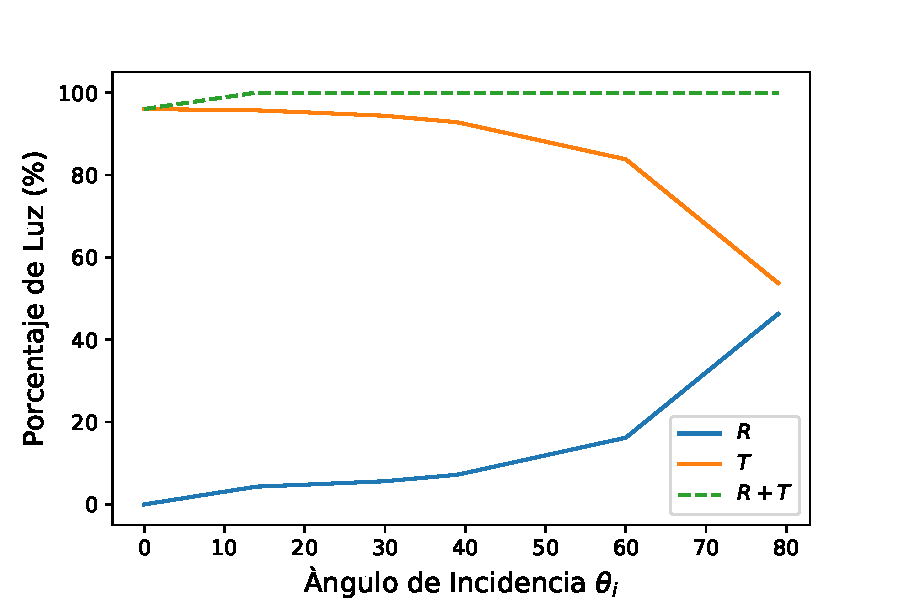
\includegraphics[width=0.9\columnwidth]{img/lab0.pdf}
\caption{\label{fig:lab0} Curvas de reflectancia y transmitancia en función del ángulo de incidencia. Para los medios: aire $\rightarrow$ vidrio; $n_i < n_t$}
\end{figure}

\begin{figure}
\centering
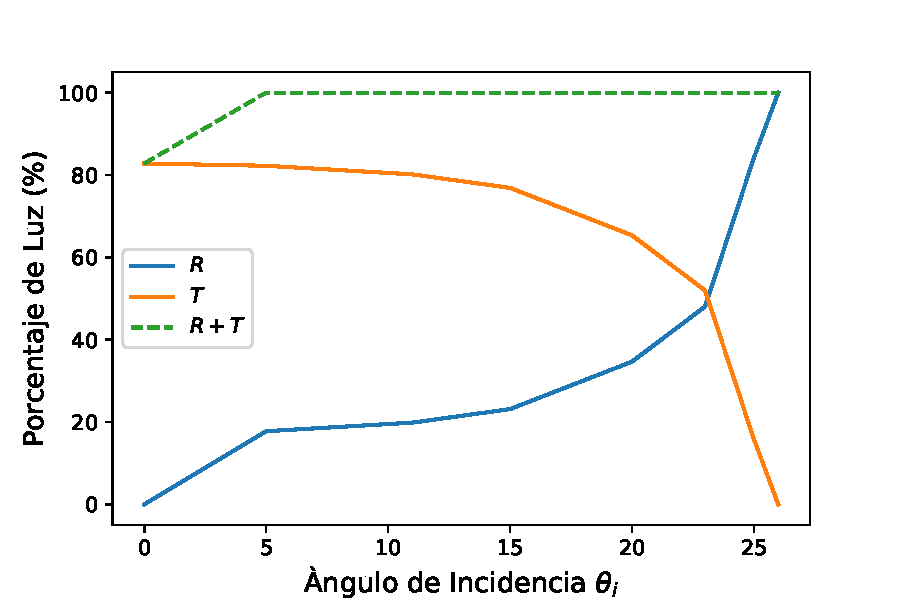
\includegraphics[width=0.9\columnwidth]{img/lab1.pdf}
\caption{\label{fig:lab1} Curvas de reflectancia y transmitancia en función del ángulo de incidencia. Para los medios: Misterio A $\rightarrow$ Aire; $n_i > n_t$}
\end{figure}


\begin{figure}
\centering
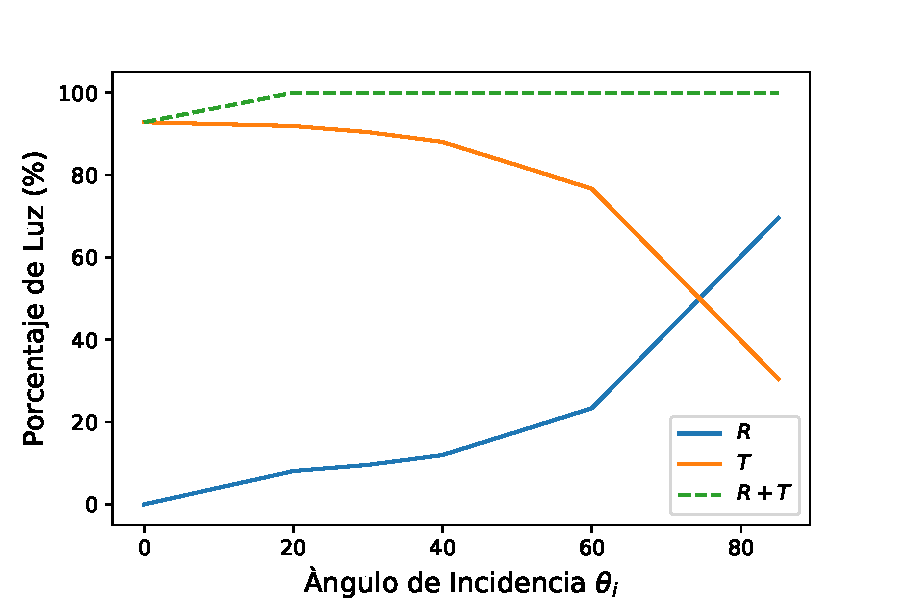
\includegraphics[width=0.9\columnwidth]{img/lab3.pdf}
\caption{\label{fig:lab2} Curvas de reflectancia y transmitancia en función del ángulo de incidencia. Para los medios: Misterio A $\rightarrow$ Misterio B; $n_i > n_t$}
\end{figure}

De modo que al observar las figuras \ref{fig:lab0}, \ref{fig:lab1} y \ref{fig:lab2}, se nota una correspondencia entre las curvas tal que $R + T = 100\% \equiv 1$. Note que generalmente, en cada gráfica, cuando el ángulo de incidencia es $0^{\circ}$, la suma de la reflectancia y la transmitancia no es ni si quiera cercano a $100\%$, esto se debe a que el medidor de intensidad del simulador Phet, al incidir el haz de forma normal a la superficie, no es capaz de medir el porcentaje de luz reflejada porque el haz incidente está superpuesto. Exceptuando este inconveniente, se comprueba la relación estudiada en la ecuación (\ref{EQN:UNIDAD}) que representa la conservación de la energía para la configuración que se muestra en la figura \ref{fig:img1}.\\

En cuanto a la amplitud de los haces reflejado y transmitido, es conveniente recordar que:

\begin{gather}
I = \frac{c \epsilon_0}{2} E_0\up{2}\\
I \propto E_0\up{2}
\end{gather}
Si la irradiancia es proporcional a la amplitud de la onda al cuadrado, podemos estimar de forma cualitativa lo que ocurre con las amplitudes a medida que se aumenta el ángulo de incidencia, de los haces reflejado y transmitido mediante las figuras \ref{fig:lab0}, \ref{fig:lab1} y \ref{fig:lab2}. En particular, bajo las condiciones de cada figura, la amplitud del haz reflejado aumenta con el ángulo de incidencia, mientras que la amplitud del haz transmitido disminuye con el ángulo de incidencia.

En cuanto a los cambios de fase, si se usa el osciloscopio en un mismo momento para comparar las fases del haz incidente y el reflejado, nos damos cuenta que ambos haces de luz se encuentran en fases opuestas. Dado que la luz del haz incidente es luz no polarizada, no es posible realizar un análisis adicional.

\section{Conclusiones}
Se concluyó que el principio de conservación de energía está presente en la configuración de un haz de luz incidente sobre una superficie que separa dos medios. La intensidad del haz incidente se distribuye en una fracción de luz reflejada y otra transmitida, de manera que la suma de estas intensidades sea igual a la inicial. Esto se cumple de manera independiente de las propiedades de los medios en el cual se propaga el haz de luz. 

\bibliography{report_physics}
\end{document}